\chapter{Processamento de Entidades Nomeadas}
\label{cap:enamex}

Entidades nomeadas são "elementos atómicos em texto" pertencentes a categorias predefinidas tais como nomes de pessoas, organizações, localizações, quantidades, etc. Assim, Processamento de Entidades Nomeadas(PEN) é a tarefa de identificar estas entidades.
Embora as categorias das entidades nomeadas serem predefinidas, existem várias opiniões sobre que categorias deve ser consideradas entidades nomeadas e quão abrangentes estas categorias devem ser. Por convenção, tags \emph{"ENAMEX"} são utilizadas para nomes, tags \emph{"NUMEX"} são utilizadas para entidades numéricas, e tags \emph{"TIMEX"} são utilizadas para entidades temporais.

Neste exercício iremos apenas processar entidades com a tag \emph{"ENAMEX"}, na forma:
\begin{itemize}
\item\verb!<ENAMEX TYPE="PERSON">Francisco de Vilela Barbosa</ENAMEX>!\\(Pessoa)
\item\verb!<ENAMEX TYPE="LOCATION" SUBTYPE="COUNTRY">Portugal</ENAMEX>!\\ (Localização, País)
\item\verb!<ENAMEX TYPE="LOCATION" SUBTYPE="CITY">Rio de Janeiro</ENAMEX>!\\  (Localização, Cidade)
\item\verb!<ENAMEX TYPE="ORGANIZATION">Universidade do Minho</ENAMEX>!\\(Organização)
\end{itemize}

Como exercício extra iremos também abordar as entidades na forma:
\begin{itemize}
\item\verb!<ENAMEX TYPE="LOCATION"> Santo Novo </ENAMEX>!\\(Localização não específica)
\end{itemize}
Todas as outras tags irão ser ignoradas.

O processamento de entidades nomeadas, apesar de ser aparentemente uma tarefa simples, enfrenta um dado numero de desafios. As entidades podem tornar-se difíceis de encontrar, e uma vez encontradas, difíceis de classificar. Localizações e nomes de pessoas podem ser as mesmas, e seguir estilos similares de formatação.

\section{Analise e Especificação}
\label{seq:enamex-ana}

Uma breve leitura do problema permite-nos entender algumas das funcionalidades necessárias, sendo estas definidas como:
\begin{itemize}
\item Necessidade de ordenação e não repetição na listagem de pessoas(alínea a): \\
	\begin{itemize}
	\item A alínea A do problema requer a listagem de todas as pessoas identificadas, sem repetições. Este informação refere-se então às tags do tipo:\\
	\verb!<ENAMEX TYPE="PERSON">...</ENAMEX>!.\\
	Por forma a armazenar e ordenar adequadamente toda a informação acerca das Pessoas, é necessária a utilização de uma estrutura capaz de suportar esta informação. 
	\end{itemize}
	
\item Listar os países e cidades marcadas (alínea b): \\
	\begin{itemize}
	\item Apesar de não estar especificado no enunciado, o grupo propôs uma implementação na qual seria possível associar cidades a certos países. Compreendemos que este tipo de implementação, para grande parte dos casos, não é viável e pode tornar a informação apresentada incoerente. No entanto, no intuito de aprender e aumentar o desafio proposto, decidimos que cidades mencionadas após países e antes de pontos finais pertenciam a esses países. Esta informação é também armazenada na estrutura implementada.
	\end{itemize}
\item Listar as organizações (alínea c): \\
	\begin{itemize}
	\item Similarmente à alínea A, a alínea C requer a listagem de todas as organizações identificadas. Esta informação refere-se então às tags do tipo: \\
	\verb! <ENAMEX TYPE="ORGANIZATION">...</ENAMEX>! \\
	E está implementada de forma similar à listagem de pessoas.
	\end{itemize}
\item Apresentar os resultados em formato HTML: \\
	\begin{itemize}
	\item Por forma a visualizar facilmente os resultados do processamento do texto, estes são apresentados em formato HTML através da implementação de funções capazes de transformar a informação contida nas estruturas em documentos de texto com o formato requerido.
	\end{itemize}
\end{itemize}

\section{Implementação}
\label{seq:enamex-imp}
\subsection{Estrutura de dados}
\label{seq:enamex-est}
Com o intuito de cumprir todos os requisitos estruturais definidos anteriormente, foi desenvolvida uma estrutura de dados única capaz de armazenar todos os dados necessários. Assim, escolhemos implementar uma árvore binária de procura, na qual os nodos possuem a informação a guardar sobre a forma de array de caracteres. A escolha desta estrutura facilita a ordenação alfabética dos diversos nomes que possamos processar, e é de implementação relativamente simples. Creemos ser superior a outras estruturas tais como listas ligadas cuja implementação, apesar de mais simples, torna-se mais complexa quando é necessária a ordenação dos seus elementos (O(N)) e a tabelas de hash cuja implementação é mais complexa, sendo que para elevadas quantidades de dados possuem ainda a necessidade de reHashing e garbage colection. 

\begin{figure}[H]
\centering
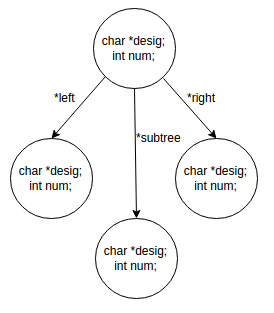
\includegraphics[width=7cm]{anexos/2-2/tree.png}
\caption{Representação gráfica da estrutura de dados}
\end{figure}

Para casos em que apenas é necessário o armazenamento da entidade, sem qualquer tipo de associação, uma árvore com dois apontadores (esquerda e direita) e com a capacidade de armazenar a informação (array de caracteres) bastaria para abordar todos os casos. No entanto, de forma a armazenar a possível associação entre os países e as suas cidades, modificamos a árvore previamente referida, e adicionamos-lhe um apontador extra, que poderá ser visto como o apontador para a raiz de uma nova árvore, constituída por todas as cidades que pertencem a um dado país. Como curiosidade, adicionamos também um inteiro em cada nodo que servirá como contador para todas as ocorrências de um dado elemento. Todo o código referente a esta estrutura encontra-se implementado no ficheiros "tree.c" e "tree.h" e pode ser consultado em anexo.

\subsection{Filtro de Texto}
\label{seq:enamex-filtro}

De forma a processar as tags pertencentes a pessoas/organizações, foram criadas expressões regulares capazes de identificar essas tags.
Assim, foram implementadas as seguintes expressões regulares para pessoas/organizações, assim como abreviaturas que facilitam a sua leitura e compreensão:

\begin{itemize}
\item pessoas: \verb! {enamex}{person}{pal}{eclose}! 
\item organizações:\verb!{enamex}{org}{pal}{eclose}!
\item localizações gerais:\verb! {enamex}{loc}{pal}{eclose}!
\item cidades: \verb!{enamex}{loc}{subcity}{pal}{eclose}!
\end{itemize}

sendo que as abreviaturas mencionadas correspondem a:

\begin{itemize}
\item Palavra \\
	\verb!    {pal} [a-zA-Z0-9Ç-ÑÀ-û ]+!
\item Tag Enamex \\
	\verb!    {enamex} \<[ \t]*(?i:enamex)[ \t]+(?i:type)=!
\item Tag de fecho \\
	\verb!    {eclose} \<[ \t]*\/(?i:enamex)[ \t]*\>!
\item Elemento "Organization"\\
	\verb!    {org} \"[ \t]*(?i:organization)[ \t]*\"[ \t]*\>!
\item Elemento "Person"\\
	\verb!    {person} \"[ \t]*(?i:person)[ \t]*\"[ \t]*\>!
\end{itemize}


De notar a capacidade das expressões regulares identificarem tags definidas tanto em letra maiuscula como minuscula, sendo também tolerantes à quantidade de espaços ou tabs presentes entre elementos destas.
De forma a implementar a capacidade de associar cidades a um dado país, foram utilizados "operadores de contexto", de forma a que caso seja detectado uma tag correspondente a um país, o analisador entre no contexto não exclusivo (\%s)country, e associa as seguintes tags correspondentes a cidades ao país em causa. Caso seja detetado um ponto final, o analisador lexico abandona esse contexto e continua a processar em contexto geral. 

\textbf{Nota}: Esta foi uma funcionalidade assumida, pelo que poderá nem sempre ter sucesso e fazer as corretas associações.

Assim as expressões regulares correspondentes a localizações/países/cidades foram definidas na forma:

\begin{itemize}
\item paises: \\
	\verb!    {enamex}{loc}{subcountry}{pal}{eclose}!
\item ponto final no contexto "country":\\
	\verb!    <country>!
\item cidades no contexto "country":\\
	\verb!    <country>{enamex}{loc}{subcity}{pal}{eclose}!
\end{itemize}

sendo que as abreviaturas mencionadas correspondem a:

\begin{itemize}
\item Elemento "Country"\\
	 \verb!    {subcountry}  (?i:subtype)=\"[ \t]*(?i:country)[ \t]*\"[ \t]*\>!
\item Elemento "City"\\
	 \verb!    {subcity} (?i:subtype)=\"[ \t]*(?i:city)[ \t]*\"[ \t]*\>!
     
\end{itemize}

Estas expressões devem encontrar-se no topo de todas as outras, devido à precedência que possuem sobre elas.

\subsection{Funcionamento}
\label{seq:enamex-func}

No cabeçalho do ficheiro flex são declarados todos os apontadores referentes às estruturas onde irá ser armazenada a informação. Existe um apontador para cada tipo de estrutura, nomeadamente: pessoas, países, cidades, organizações e outras localizações. São também declarados dois apontadores para arrays de caracteres que irão auxiliar o processamento das expressões capturadas. Após início do programa, é efetuada a chamada ao analisador léxico, responsável por capturar os dados referentes às expressões definidas. Cada vez que este efetua uma captura, estes dados são processados, sendo inseridos na estrutura correspondente, sendo que caso necessário lhes são retirados os espaços em branco que possam ter antes e depois da seu conteúdo, por forma a evitar inconsistência de dados. Após o término da leitura do input em questão, todos os dados presentes nas estruturas são escritos nos ficheiros HTML correspondentes, estando estes interligados através de hiperligações (tags <a href=""/>). Cada estrutura (tipo de entidade) é escrita em ficheiro através da função treeToHTML (implementada no ficheiro tree.c), responsável por receber como parâmetros um apontador para estrutura e um identificador de ficheiro (previamente declarado), e transferir a informação para o ficheiro no formato adequado.

\begin{figure}[H]
\centering
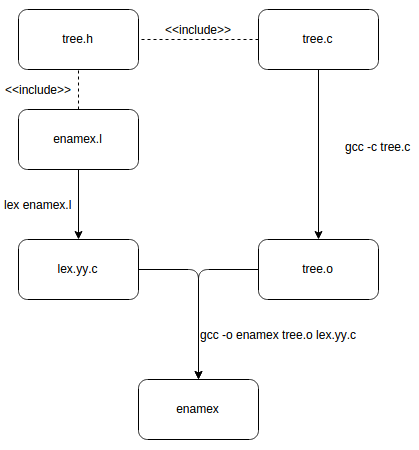
\includegraphics[width=7cm]{anexos/2-2/programa.png}
\caption{Componentes do programa}
\end{figure}
\section{Testes realizados}
\label{seq:enamex-test}
Estão documentados neste secção 3 testes realizados ao autómato, utilizando como input os ficheiros que se encontram em anexo: \ref{seq:anex-enamex-test-in01}, \ref{seq:anex-enamex-test-in02} e \ref{seq:anex-enamex-test-in03}.

\subsubsection{Teste nº 1}

Teste focado na funcionalidade de associar diversas cidades a um dado país. Como é possível verificar em anexo, o resultado é uma conexão entre "Portugal" e algumas das suas cidades.

\subsubsection{Teste nº 2}

Teste exemplificado no enunciado. Processado de acordo com o esperado (exemplo da página referente aos locais).

\subsubsection{Teste nº 3}

Teste obtido de um caso real, e focado nas tags de organizações. Resultado correto.


% respectivo enunciado da descricao do problema, das decisoes que lideraram o desenho da solucao e sua implementacao  (incluir a especificacao Flex , deverao conter exemplos de utilizacao (textos fontes diversos e respectivo resultado produzido).

% conceção e arquitetura do sistema

% testes antes da conclusao e intercalar imagens com o texto

% código em apendice em anexo

% dificuldades e decisões antes do código

% imagens bem descritas por texto

% Problema->decisão->solução

% analise e especificação é depois da descrição do problema

% análise: pega nisto, faz isto
% (descascar o problema)=> resultado(especificação) temos isto e dá isto


% respectivo enunciado da descricao do problema, => A introdução depois do titulo 
% as decisoes que lideraram o desenho da solucao e sua implementacao  => estrutura de dados
% (incluir a especificacao Flex ,                       => filtro de texto
% deverao conter exemplos de utilizacao (textos fontes diversos e respectivo resultado produzido) => exemplos